\documentclass[aspectratio=169,10pt]{beamer}
\usetheme{Madrid}
\usecolortheme{seahorse}

\usepackage{amsmath}
\usepackage{amssymb}
\usepackage{amsthm}
\usepackage{graphicx}
\usepackage{listings}
\usepackage{xcolor}
\usepackage{fancybox}

\graphicspath{{figures/}}

% Define colors for code
\definecolor{darkgreen}{rgb}{0,0.5,0}
\definecolor{darkblue}{rgb}{0,0,0.5}
\definecolor{darkred}{rgb}{0.5,0,0}

% Listings style
\lstset{
    basicstyle=\ttfamily\scriptsize,
    keywordstyle=\color{darkblue}\bfseries,
    commentstyle=\color{darkgreen}\itshape,
    stringstyle=\color{darkred},
    breaklines=true,
    breakatwhitespace=true,
    numbers=left,
    numberstyle=\tiny\color{gray},
    frame=single,
    backgroundcolor=\color{gray!5},
    showstringspaces=false,
    tabsize=2,
    captionpos=b
}

\setbeamertemplate{footline}[frame number]
\setbeamertemplate{navigation symbols}{}

\title{Chapter 9d: Applications of Fixed Point Theorems}
\subtitle{Nonlinear Analysis and Fixed Point Theory}
\author{Based on H. K. Pathak (2018)}
\date{\today}

\begin{document}

\frame{\titlepage}

% ============================================================================
% CHAPTER OVERVIEW
% ============================================================================
\section{Chapter Overview}

\begin{frame}
    \frametitle{Chapter 9d: Applications of Fixed Point Theorems}
    \begin{center}
        
\includegraphics[width=0.9\textwidth]{chapter_overview}
    \end{center}
    \vspace{-5mm}
    \begin{itemize}
        \item Applications to Volterra integrodifferential equations
        \item Applications to surjectivity of nonlinear operators
        \item Applications to complementarity problems
        \item Generalized directional contractors
    \end{itemize}
\end{frame}

\begin{frame}
    \frametitle{Key Sections in Chapter 9d}
    \begin{enumerate}
        \item \textbf{Section 9.6:} Applications to Abstract Volterra Integrodifferential Equations
        \item \textbf{Section 9.7:} Applications to Surjectivity Theorems
        \item \textbf{Section 9.8:} Applications to Simultaneous Complementarity Problems
        \item \textbf{Section 9.9:} Generalized Directional Contractors
        \item \textbf{Exercises:} 9.1 - 9.7
    \end{enumerate}
    \bigskip
    \textbf{Main Focus:} Practical applications of fixed point theorems to important problems in analysis
\end{frame}

% ============================================================================
% SECTION 9.6: VOLTERRA INTEGRODIFFERENTIAL EQUATIONS
% ============================================================================
\section{Applications to Volterra Equations}

\begin{frame}
    \frametitle{Section 9.6: Volterra Integrodifferential Equations}

    \textbf{Background:} Volterra integral equations describe many physical phenomena including
    \begin{itemize}
        \item Hereditary systems
        \item Systems with memory effects
        \item Viscoelastic materials
        \item Population dynamics
    \end{itemize}

    \bigskip

    \textbf{Standard Volterra Equation:}
    \[
    x(t) = x_0 + \int_0^t a(s)x(s)ds + \int_0^t a(s)\left(\int_0^s b(r)x(r)dr\right) ds + \cdots
    \]
\end{frame}

\begin{frame}
    \frametitle{Key Lemmas for Volterra Equations}

    \begin{block}{Lemma 9.4 (Common Fixed Point)}
        Let $T_1$ and $T_2$ be maps on complete metric space $X$. If there exists positive integer $m$ and $k < 1$ such that
        \[
        d(T_1^m x, T_2^m y) \leq kd(x,y) \quad \forall x,y \in X
        \]
        then $T_1$ and $T_2$ have a unique common fixed point.
    \end{block}

    \bigskip

    \begin{block}{Lemma 9.5 (Pachpatte's Inequality)}
        Let $x(t), a(t), b(t), c(t)$ be real-valued nonnegative continuous functions. If
        \[
        x(t) \leq x_0 + \int_0^t a(s)x(s)ds + \cdots
        \]
        then
        \[
        x(t) \leq x_0\left(1 + \int_0^t a(s)\exp\left(\int_s^t a(r)dr\right)ds\right)
        \]
    \end{block}
\end{frame}

\begin{frame}
    \frametitle{Theorem 9.34: Solution of Volterra Equations}

    \begin{block}{Theorem 9.34 (Pathak)}
        Suppose conditions $A_1$--$A_3$ are satisfied. Then for $u_0 \in B$, the initial value problems
        \[
        \begin{cases}
            (Fu)(t) = H(T, t_0, f, g, h, K_1, K_2) & t_0 \leq t < \infty \\
            (\bar{F}u)(t) = H(T, t_0, \bar{f}, \bar{g}, \bar{h}, \bar{K}_1, \bar{K}_2) & t_0 \leq t < \infty
        \end{cases}
        \]
        have a unique common mild solution $u(t)$ in $C([t_0, t_1], B)$ for $t \geq t_0$, where $t_1$ is arbitrary with $t_1 > t_0$.
    \end{block}

    \bigskip

    \begin{alertblock}{Proof Idea}
        \begin{itemize}
            \item Define norm on Banach space
            \item Show $F$ and $\bar{F}$ are contraction mappings
            \item Apply common fixed point theorem
        \end{itemize}
    \end{alertblock}
\end{frame}

\begin{frame}[fragile]
    \frametitle{Numerical Example: Volterra Equation}

    \textbf{Problem:} Solve $x(t) = 1 + \int_0^t x(s)ds$ on $[0, 1]$

    \bigskip

    \begin{lstlisting}[language=Python, caption=Volterra Equation Solver]
import numpy as np
from scipy.integrate import odeint

def volterra_example():
    # Kernel: K(t,s) = 1 (exponential kernel)
    def kernel(t, s):
        return 1.0

    # Iterative solution
    x = lambda t: 1.0  # Initial guess

    for iteration in range(10):
        # Update using Picard iteration
        x_new = lambda t: 1.0 + np.trapz(
            [x(s) for s in np.linspace(0, t, 50)],
            np.linspace(0, t, 50))
        x = x_new

    # Exact solution: x(t) = e^t
    t_vals = np.linspace(0, 1, 100)
    x_exact = np.exp(t_vals)

    return t_vals, x_exact
    \end{lstlisting}
\end{frame}

\begin{frame}
    \frametitle{Volterra Equations: Graphical Illustration}

    \begin{center}
        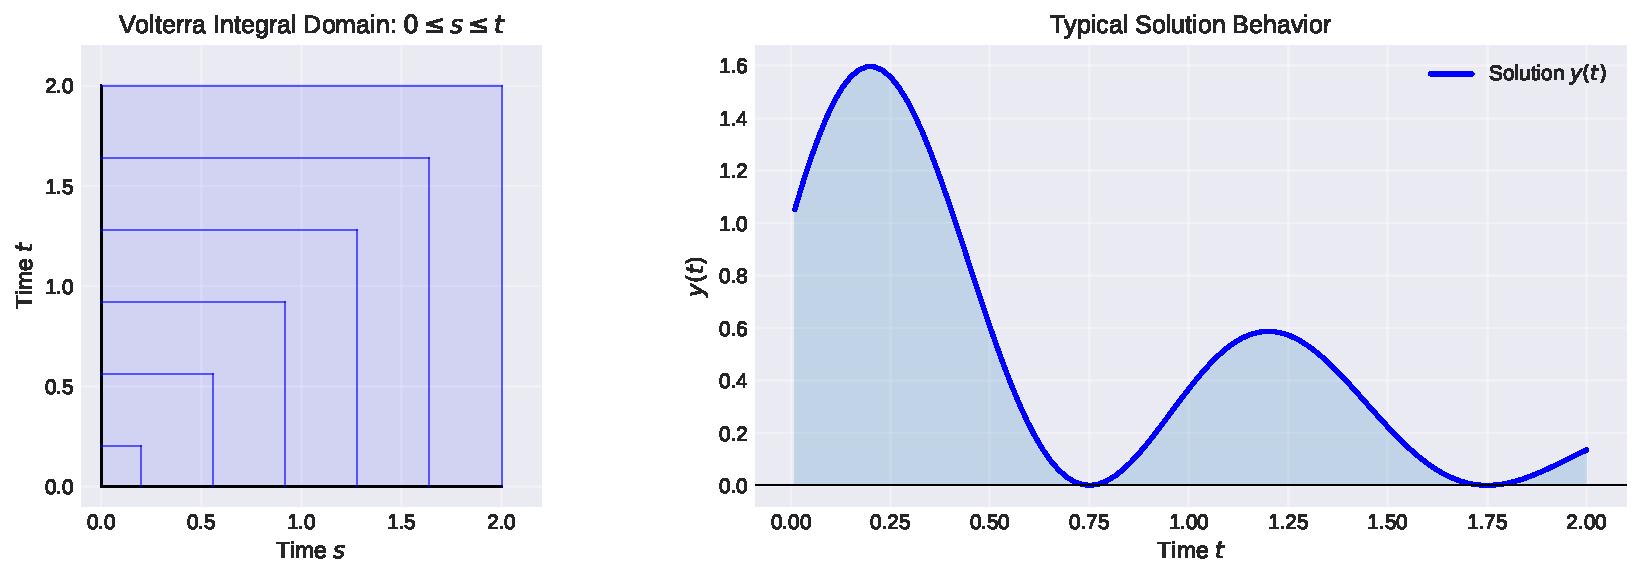
\includegraphics[width=0.9\textwidth]{volterra_structure}
    \end{center}

    \vspace{-3mm}
    \small
    \textbf{Left:} Integration domain for Volterra equations \\
    \textbf{Right:} Typical solution behavior with exponential decay
\end{frame}

% ============================================================================
% SECTION 9.7: SURJECTIVITY THEOREMS
% ============================================================================
\section{Surjectivity Theorems}

\begin{frame}
    \frametitle{Section 9.7: Applications to Surjectivity Theorems}

    \textbf{Problem:} Under what conditions is operator $P: \mathcal{D}(P) \to Y$ surjective?

    \bigskip

    \begin{definition}
        A mapping $P: X \to Y$ is \textbf{surjective} if for every $y \in Y$, there exists $x \in X$ such that $P(x) = y$.
    \end{definition}

    \bigskip

    \begin{itemize}
        \item Classical surjectivity theorems apply only to linear operators
        \item Extension to nonlinear operators requires new techniques
        \item Fixed point methods provide powerful tools
    \end{itemize}
\end{frame}

\begin{frame}
    \frametitle{Directional Contractors}

    \begin{definition}
        Let $P: \mathcal{D}(P) \subset X \to Y$. The mapping $\Gamma: \mathcal{D}(P) \to \mathcal{D}(P)$ is a \textbf{directional contractor} for $P$ if there exists $q = q(P) < 1$ and $\varepsilon = \varepsilon(x,y) \in (0,1]$ such that
        \[
        \|P(x + \varepsilon\Gamma(x)y) - Px - \varepsilon y\| \leq q\varepsilon\|y\|
        \]
    \end{definition}

    \bigskip

    \begin{definition}
        $\Gamma$ is a \textbf{generalized directional contractor} if
        \[
        \|P(x + \varepsilon\Gamma(x)y) - Px - \varepsilon y\| \leq q\varepsilon c(\|x\|)\|y\|
        \]
        where $c: [0,\infty) \to (0, q^{-1/2})$ is nonincreasing.
    \end{definition}
\end{frame}

\begin{frame}
    \frametitle{Theorem 9.37: Surjectivity via Directional Contractors}

    \begin{block}{Theorem 9.37}
        Let $X$ and $Y$ be two Banach spaces. A nonlinear map $P: \mathcal{D}(P) \subset X \to Y$ which has closed graph and a bounded generalized directional contractor $\Gamma$ is surjective.
    \end{block}

    \bigskip

    \begin{alertblock}{Proof Strategy}
        \begin{enumerate}
            \item Define metric $\rho(x,y) = \max\{\|x-y\|, (1+q^{1/2})^{-1}\|Px - Py\|\}$ on $\mathcal{D}(P)$
            \item Show $(\mathcal{D}(P), \rho)$ is complete metric space
            \item Construct contractive iterative process
            \item Use fixed point theorem to prove existence
        \end{enumerate}
    \end{alertblock}
\end{frame}

\begin{frame}
    \frametitle{Application to Specific Problems}

    \textbf{Example 1: Nonlinear Integral Equation}
    \[
    u(t) = h(t) + \int_0^t K(t,s)u(s)ds
    \]

    \textbf{Surjectivity:} For given $h \in L^p[0,T]$, does a solution exist?

    \bigskip

    \textbf{Example 2: Boundary Value Problem}
    \[
    -u'' = f(t, u(t)), \quad u(0) = u(1) = 0
    \]

    \textbf{Question:} Is the Green's operator surjective onto appropriate function spaces?

    \bigskip

    \begin{itemize}
        \item Use directional contractor to establish surjectivity
        \item Guarantee existence of solutions for all right-hand sides
        \item Extend to nonlinear settings
    \end{itemize}
\end{frame}

\begin{frame}
    \frametitle{Surjectivity and Fixed Points}

    \begin{center}
        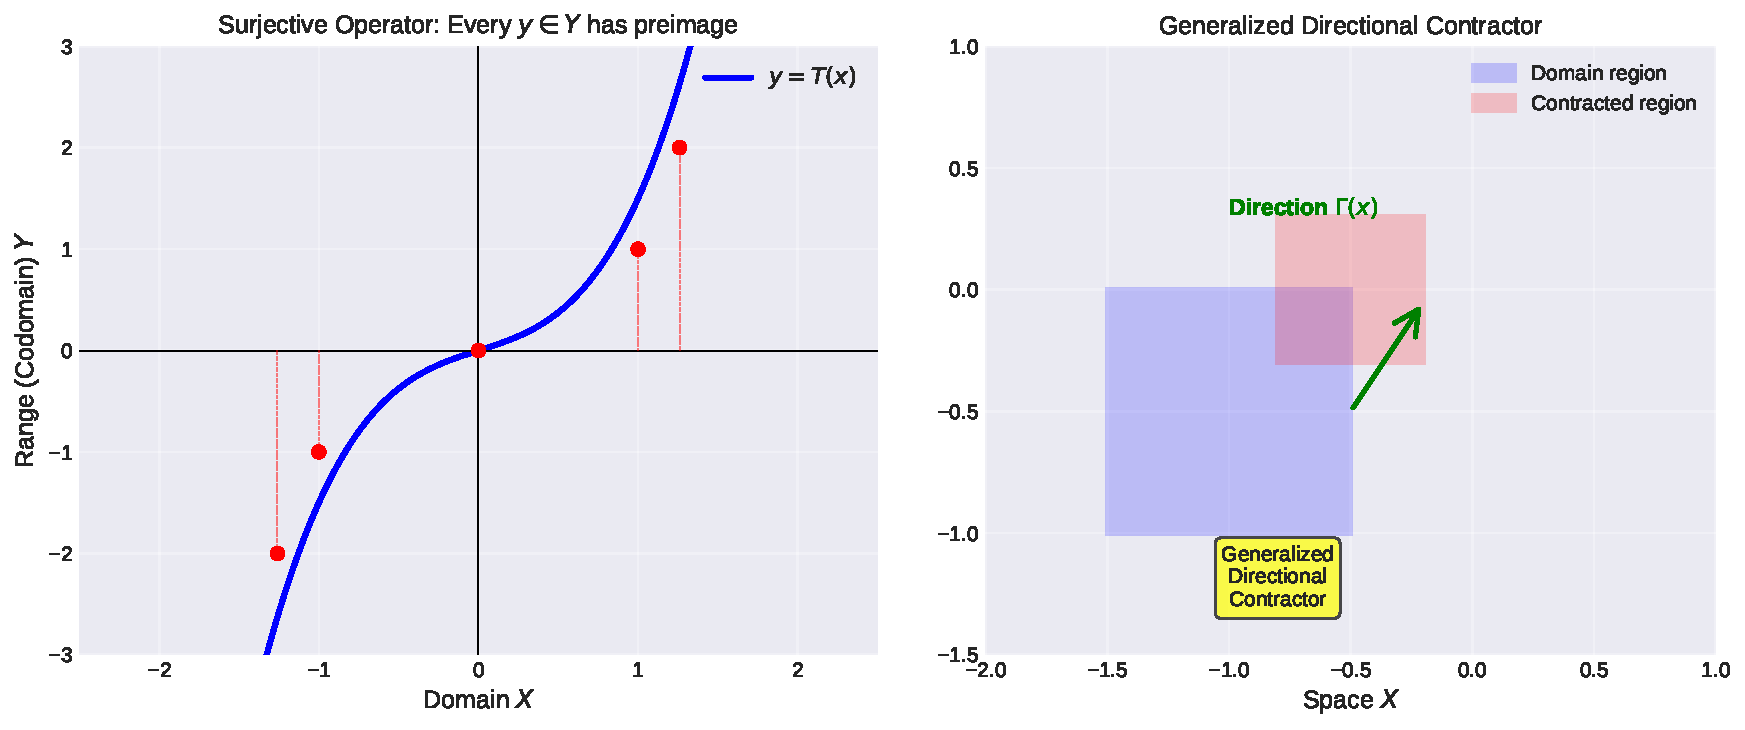
\includegraphics[width=0.95\textwidth]{surjectivity_application}
    \end{center}

    \vspace{-3mm}
    \small
    \textbf{Left:} Surjective operator mapping domain to full codomain \\
    \textbf{Right:} Generalized directional contractor with contraction property
\end{frame}

% ============================================================================
% SECTION 9.8: COMPLEMENTARITY PROBLEMS
% ============================================================================
\section{Complementarity Problems}

\begin{frame}
    \frametitle{Section 9.8: Complementarity Problems}

    \textbf{Background:} Complementarity problems arise in
    \begin{itemize}
        \item Optimization and mathematical programming
        \item Mechanics (contact problems, friction)
        \item Economics (equilibrium problems)
        \item Game theory
        \item Traffic flow and network analysis
    \end{itemize}

    \bigskip

    \textbf{Historical Note:} First studied systematically in 1960s by Lemke and Howson
\end{frame}

\begin{frame}
    \frametitle{Explicit Complementarity Problem (ECP)}

    \begin{definition}
        \textbf{Explicit Complementarity Problem (ECP):} Find $x_0 \in K$ such that $f(x_0) \in K^*$ and $\langle x_0, f(x_0) \rangle = 0$, where
        \begin{itemize}
            \item $(E, E^*)$ is a dual system of locally convex spaces
            \item $K$ is a closed convex cone in $E$
            \item $K^* = \{u \in E^* : \langle x, u \rangle \geq 0 \text{ for all } x \in K\}$ is dual cone
            \item $f: K \to E^*$ is mapping
        \end{itemize}
    \end{definition}

    \bigskip

    \textbf{Notation:} $0 \leq x_0 \perp f(x_0) \geq 0$ (orthogonal complementarity)
\end{frame}

\begin{frame}
    \frametitle{Implicit Complementarity Problem (ICP)}

    \begin{definition}
        \textbf{Implicit Complementarity Problem (ICP):} Find $x_0 \in K$ such that $\langle x_0, g(x_0) \rangle = 0$ where
        \begin{itemize}
            \item $g: K \to E^*$ is a mapping
            \item Solution must satisfy additional constraints
        \end{itemize}
    \end{definition}

    \bigskip

    \begin{block}{Relationship Between ECP and ICP}
        \begin{itemize}
            \item ICP is more general than ECP
            \item ICP can model implicit functional constraints
            \item Both require finding orthogonal pairs in cone-dual cone structure
        \end{itemize}
    \end{block}
\end{frame}

\begin{frame}
    \frametitle{Linear Complementarity Problem (LCP)}

    \begin{definition}
        \textbf{Linear Complementarity Problem (LCP):} Find $x \in \mathbb{R}^n$ such that
        \[
        \begin{cases}
            0 \leq x \\
            0 \leq Mx + q \\
            \langle x, Mx + q \rangle = 0
        \end{cases}
        \]
        where $M \in \mathbb{R}^{n \times n}$ and $q \in \mathbb{R}^n$.
    \end{definition}

    \bigskip

    \textbf{Notation:} $\text{LCP}(M, q)$

    \bigskip

    \begin{alertblock}{Special Cases}
        \begin{itemize}
            \item If $M$ is positive definite: unique solution
            \item If $M$ is monotone: solution may not be unique but existence guaranteed
            \item General $M$: solution may not exist
        \end{itemize}
    \end{alertblock}
\end{frame}

\begin{frame}
    \frametitle{Complementarity Problem Geometry}

    \begin{center}
        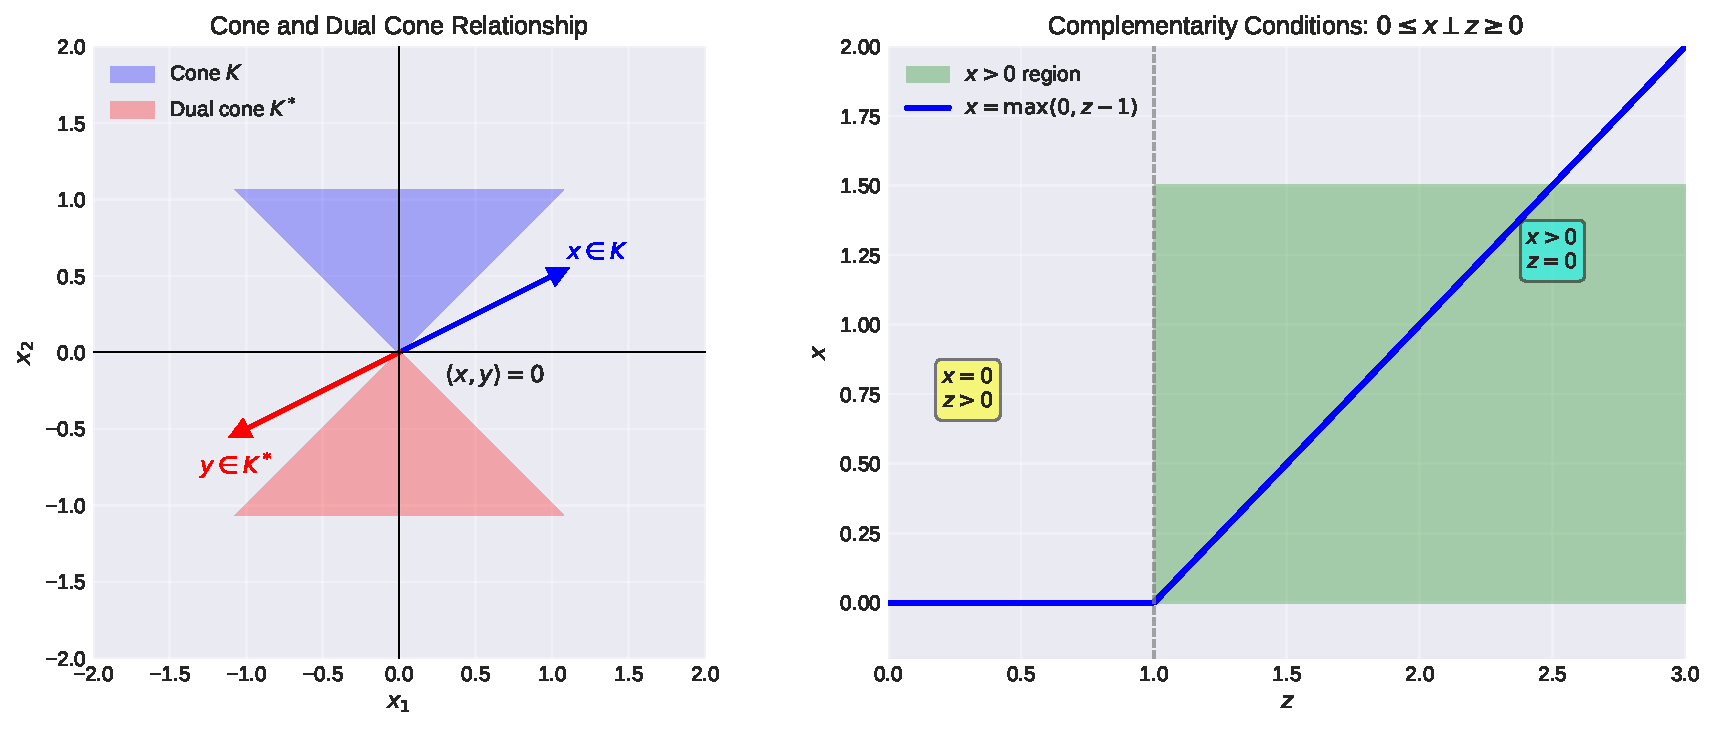
\includegraphics[width=0.95\textwidth]{complementarity_problem}
    \end{center}

    \vspace{-3mm}
    \small
    \textbf{Left:} Cone and dual cone relationship with orthogonality \\
    \textbf{Right:} Complementarity condition: $x \geq 0 \perp z \geq 0$
\end{frame}

\begin{frame}[fragile]
    \frametitle{Numerical Solution: LCP Example}

    \textbf{Problem:} Solve $\text{LCP}(M, q)$ where
    \[
    M = \begin{pmatrix} 2 & 1 \\ 1 & 2 \end{pmatrix}, \quad q = \begin{pmatrix} -3 \\ -3 \end{pmatrix}
    \]

    \begin{lstlisting}[language=Python, caption=Lemke Algorithm]
import numpy as np

def lemke_method(M, q, max_iter=1000):
    n = len(q)
    x = np.zeros(n)
    s = -q.copy()

    for iteration in range(max_iter):
        # Find entering variable
        if np.all(s >= 0):
            return x  # Feasible solution found

        j = np.argmin(s)  # Most negative slack

        # Update using complementarity
        x[j] += s[j] / M[j, j]
        s = -q - M @ x

    return x

# Solve
x_sol = lemke_method(M, q)
print(f"Solution: x = {x_sol}")
print(f"Residual: ||Mx + q|| = {np.linalg.norm(M @ x_sol + q)}")
    \end{lstlisting}
\end{frame}

% ============================================================================
% SECTION 9.9: DIRECTIONAL CONTRACTORS
% ============================================================================
\section{Generalized Directional Contractors}

\begin{frame}
    \frametitle{Definition 9.9: Generalized Directional Contractor}

    \begin{definition}
        Let $X$ and $Y$ be Banach spaces, $P: \mathcal{D}(P) \subset X \to Y$ a nonlinear operator from linear subspace $\mathcal{D}(P)$ of $X$ to $Y$, and $\Gamma: \mathcal{D}(P) \to \mathcal{D}(P)$ a bounded linear operator. A positive number $q = q(P) < 1$ exists such that for any $x \in \mathcal{D}(P)$ and $y \in Y$, there exist $\varepsilon = \varepsilon(x,y) \in (0,1]$ and a nonincreasing function $c: [0,\infty) \to (0, q^{-1/2})$ satisfying
        \[
        \|P(x + \varepsilon\Gamma(x)y) - Px - \varepsilon y\| \leq q\varepsilon c(\|x\|)\|y\|
        \]
        Then $\Gamma(x)$ is called a \textbf{generalized directional contractor} for $P$ at $x \in \mathcal{D}(P)$.
    \end{definition}
\end{frame}

\begin{frame}
    \frametitle{Properties of Directional Contractors}

    \begin{theorem}
        For a generalized directional contractor $\Gamma$:
        \begin{enumerate}
            \item If $\Gamma(x)y = 0$, then $y = 0$ (injectivity)
            \item $\Gamma$ is bounded: $\|\Gamma(x)\| \leq B$ for some constant $B > 0$
            \item $\Gamma(x)$ measures the "direction" of steepest descent for $P$
            \item Inverse operator approximated by directional contractor
        \end{enumerate}
    \end{theorem}

    \bigskip

    \begin{block}{Key Observation}
        Every inverse Fréchet derivative is a directional contractor, and every generalized directional contractor is a directional contractor.
    \end{block}
\end{frame}

\begin{frame}
    \frametitle{Applications of Directional Contractors}

    \begin{block}{Application 1: Surjectivity}
        Use directional contractor to prove surjectivity of operators with closed graph
    \end{block}

    \begin{block}{Application 2: Implicit Function Theorem}
        Establish implicit function theorems for operators admitting directional contractors
    \end{block}

    \begin{block}{Application 3: Variational Inequalities}
        Solve variational inequalities of form:
        \[
        \langle P(x), y - x \rangle \geq f(y) - f(x) \quad \forall y \in K
        \]
    \end{block}

    \begin{block}{Application 4: Nonlinear Equations}
        Solve $P(x) = 0$ where $P$ has directional contractor
    \end{block}
\end{frame}

\begin{frame}
    \frametitle{Fixed Point Geometry}

    \begin{center}
        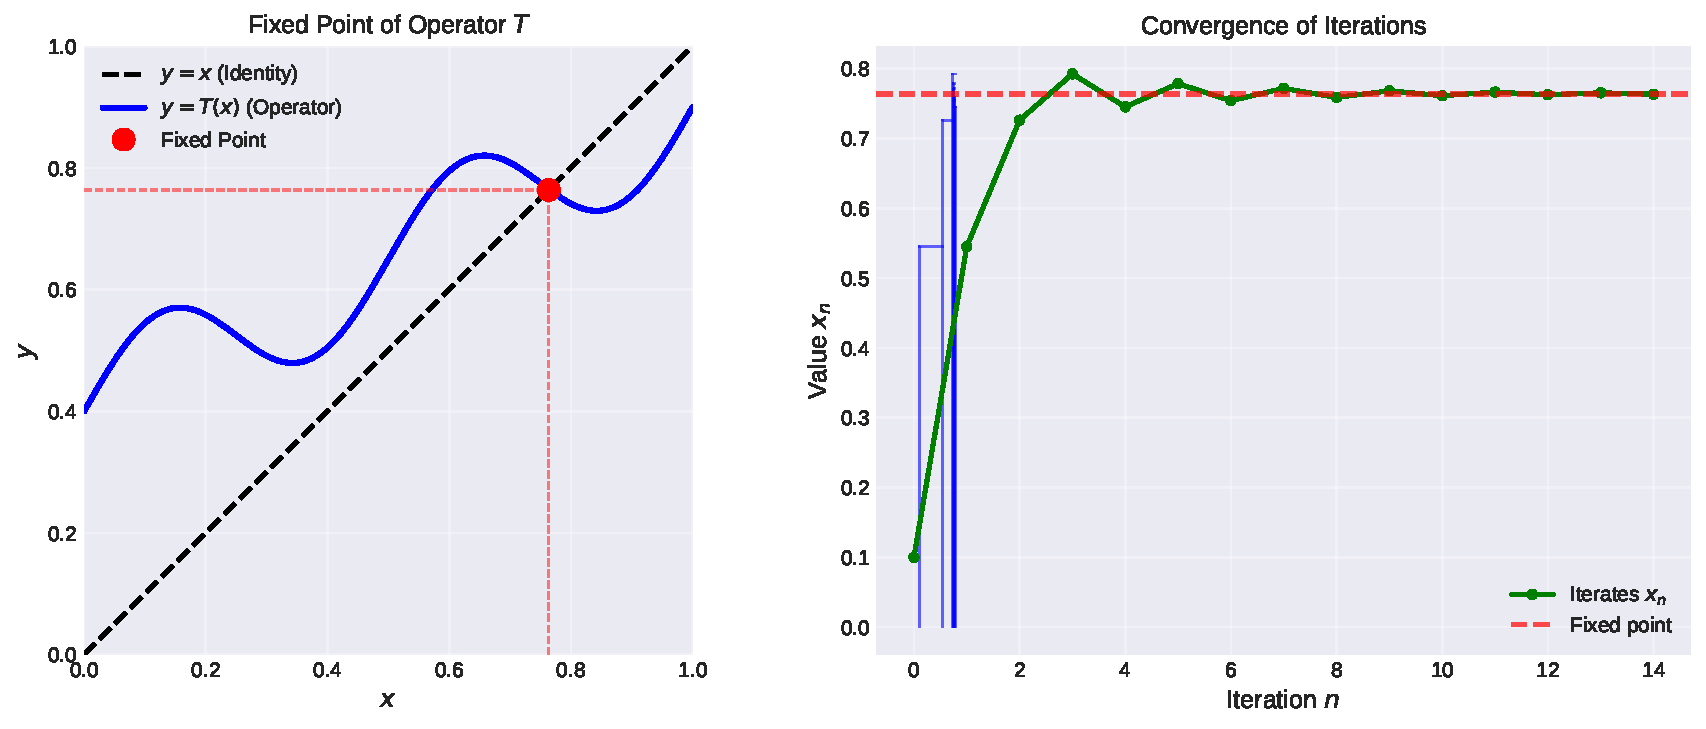
\includegraphics[width=0.95\textwidth]{fixed_point_geometry}
    \end{center}

    \vspace{-3mm}
    \small
    \textbf{Left:} Intersection of function with identity line defines fixed point \\
    \textbf{Right:} Iterative convergence to fixed point under contraction
\end{frame}

% ============================================================================
% FIXED POINT THEORY FOUNDATIONS
% ============================================================================
\section{Fixed Point Theory Background}

\begin{frame}
    \frametitle{Banach Contraction Mapping Principle}

    \begin{theorem}[Banach]
        Let $(X, d)$ be a complete metric space and $T: X \to X$ a mapping such that
        \[
        d(T(x), T(y)) \leq kd(x,y) \quad \forall x, y \in X
        \]
        for some $k \in [0,1)$. Then:
        \begin{enumerate}
            \item $T$ has a unique fixed point $x^* \in X$
            \item The sequence $\{x_n\}$ defined by $x_{n+1} = T(x_n)$ converges to $x^*$ for any $x_0 \in X$
            \item Error estimate: $d(x_n, x^*) \leq k^n d(x_0, x^*)$
        \end{enumerate}
    \end{theorem}

    \bigskip

    \begin{alertblock}{Why Important for Chapter 9d?}
        All applications rely on this fundamental principle by constructing appropriate operators and metrics
    \end{alertblock}
\end{frame}

\begin{frame}
    \frametitle{Contraction Mapping Convergence Rates}

    \begin{center}
        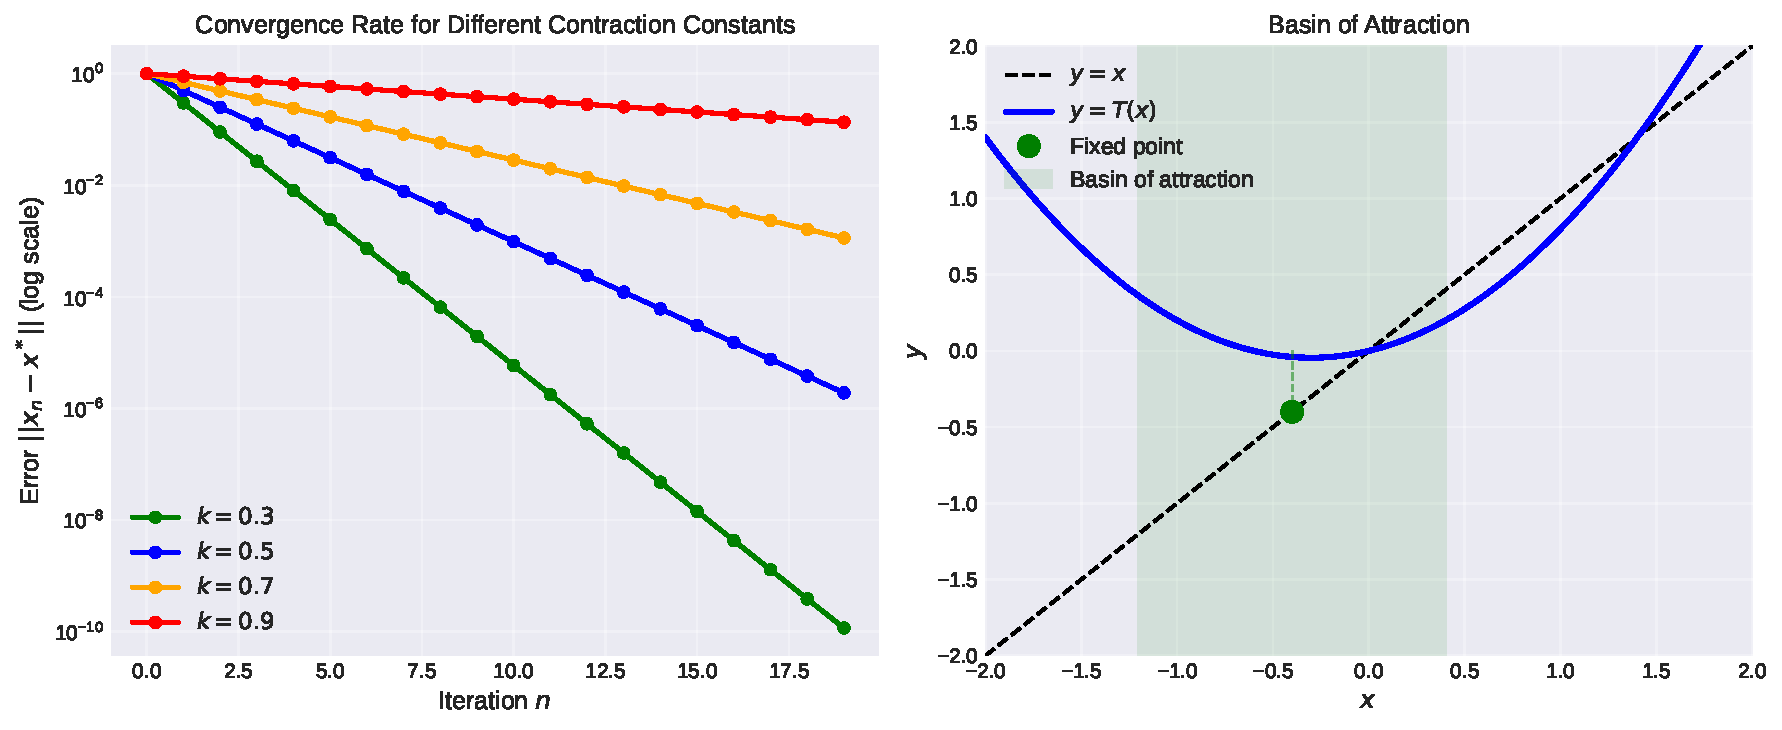
\includegraphics[width=0.95\textwidth]{contraction_mapping_rate}
    \end{center}

    \vspace{-3mm}
    \small
    \textbf{Left:} Error decreases exponentially with iteration number \\
    \textbf{Right:} Basin of attraction around fixed point
\end{frame}

\begin{frame}[allowframebreaks]
    \frametitle{Conditions for Fixed Point Existence}

    \begin{block}{Condition 1: Complete Metric Space}
        $(X, d)$ must be complete. Alternatively, use Banach spaces with
        \begin{itemize}
            \item Closed subsets (complete)
            \item Natural metrics
        \end{itemize}
    \end{block}

    \begin{block}{Condition 2: Contraction Property}
        Need $d(T(x), T(y)) \leq kd(x,y)$ with $k < 1$. This can be:
        \begin{itemize}
            \item Uniform contraction
            \item Lipschitz continuous mapping
            \item Operator norm condition
        \end{itemize}
    \end{block}

    \begin{block}{Condition 3: Appropriate Metric}
        Choice of metric is crucial:
        \begin{itemize}
            \item Standard metric: $d(x,y) = \|x - y\|$
            \item Weighted metric: $\rho(x,y) = w(x,y)\|x-y\|$
            \item Custom metric tailored to problem
        \end{itemize}
    \end{block}

    \framebreak

    \begin{block}{Metric Construction in Chapter 9d}
        For surjectivity problems:
        \[
        \rho(x,y) = \max\{\|x-y\|, (1+q^{1/2})^{-1}\|Px - Py\|\}
        \]
        This metric makes $(\mathcal{D}(P), \rho)$ complete when original space isn't!
    \end{block}
\end{frame}

% ============================================================================
% COMPARISON WITH OTHER METHODS
% ============================================================================
\section{Comparison and Extensions}

\begin{frame}
    \frametitle{Fixed Point Methods vs. Optimization Methods}

    \begin{table}
        \centering
        \small
        \begin{tabular}{|l|c|c|c|}
            \hline
            \textbf{Property} & \textbf{Fixed Point} & \textbf{Newton} & \textbf{Gradient Descent} \\
            \hline
            Convergence Rate & Linear & Quadratic & Sublinear \\
            \hline
            Derivative Needed & Yes/No & Yes & Yes \\
            \hline
            Stability & Global & Local & Slow \\
            \hline
            Complexity/Iter & Low & High & Low \\
            \hline
            Nonlinear Problems & Yes & Yes & Limited \\
            \hline
        \end{tabular}
    \end{table}

    \bigskip

    \begin{block}{Fixed Point Advantages}
        \begin{itemize}
            \item Works without derivative information
            \item Global convergence under weak conditions
            \item Applicable to wide class of problems
        \end{itemize}
    \end{block}
\end{frame}

\begin{frame}
    \frametitle{Extensions Beyond Chapter 9d}

    \begin{itemize}
        \item \textbf{Partial Metric Spaces:} Generalization for distance to self not necessarily zero

        \item \textbf{Fuzzy Metric Spaces:} Probabilistic distances between points

        \item \textbf{Multivalued Maps:} Fixed point results for set-valued operators

        \item \textbf{Fractional Operators:} Application to fractional differential equations

        \item \textbf{Variational Inclusions:} Generalizations to inclusion problems

        \item \textbf{Metric-like Spaces:} Weaker distance axioms but stronger theorems
    \end{itemize}
\end{frame}

% ============================================================================
% PRACTICAL APPLICATIONS
% ============================================================================
\section{Practical Applications}

\begin{frame}[allowframebreaks]
    \frametitle{Real-World Applications}

    \begin{block}{1. Mechanical Systems}
        \begin{itemize}
            \item Vibration problems with friction and damping
            \item Contact mechanics and Coulomb friction
            \item Elastic-plastic deformations
        \end{itemize}
    \end{block}

    \begin{block}{2. Economic Equilibrium}
        \begin{itemize}
            \item Supply-demand equilibrium
            \item Nash equilibrium in games
            \item Market clearing conditions
        \end{itemize}
    \end{block}

    \framebreak

    \begin{block}{3. Systems with Memory}
        \begin{itemize}
            \item Viscoelastic materials
            \item Biological systems with hereditary effects
            \item Chemical reactions with memory terms
        \end{itemize}
    \end{block}

    \begin{block}{4. Traffic Flow and Networks}
        \begin{itemize}
            \item Network flow problems
            \item User equilibrium on transportation networks
            \item Network design optimization
        \end{itemize}
    \end{block}
\end{frame}

\begin{frame}[fragile]
    \frametitle{Practical Implementation Example}

    \begin{lstlisting}[language=Python, caption=Fixed Point Iteration Solver]
import numpy as np

def fixed_point_solver(T, x0, tol=1e-8, max_iter=1000):
    """
    Solve x = T(x) using fixed point iteration

    Args:
        T: Function defining the fixed point operator
        x0: Initial guess
        tol: Convergence tolerance
        max_iter: Maximum iterations

    Returns:
        x_star: Fixed point solution
    """
    x = x0
    history = [x.copy()]

    for iteration in range(max_iter):
        x_new = T(x)
        error = np.linalg.norm(x_new - x)
        history.append(x_new.copy())

        if error < tol:
            print(f"Converged in {iteration} iterations")
            return x_new, np.array(history)

        x = x_new

    print(f"Warning: max iterations reached")
    return x, np.array(history)

# Example: Solve x = 0.5*sin(x) + 0.3
T = lambda x: 0.5*np.sin(x) + 0.3
x_sol, hist = fixed_point_solver(T, x0=np.array([0.0]))
print(f"Solution: x = {x_sol}")
    \end{lstlisting}
\end{frame}

% ============================================================================
% KEY THEOREMS SUMMARY
% ============================================================================
\section{Summary of Key Theorems}

\begin{frame}[allowframebreaks]
    \frametitle{Summary: Theorems in Chapter 9d}

    \begin{block}{Theorem 9.34}
        \textbf{Volterra Equations:} Existence and uniqueness of common mild solution for two operators satisfying contraction property on appropriate Banach space.
    \end{block}

    \begin{block}{Theorem 9.37}
        \textbf{Surjectivity:} Nonlinear operator with closed graph and bounded generalized directional contractor is surjective onto $Y$.
    \end{block}

    \framebreak

    \begin{block}{Theorems 9.38-9.40}
        \textbf{Complementarity:} Existence results for explicit and implicit complementarity problems using fixed point theory and monotone operator theory.
    \end{block}

    \begin{block}{Definition 9.9}
        \textbf{Generalized Directional Contractor:} Extension of classical directional contractor with function-valued contraction constant.
    \end{block}
\end{frame}

\begin{frame}
    \frametitle{Proof Techniques Used}

    \begin{enumerate}
        \item \textbf{Metric Construction:} Create custom metrics to ensure completeness and contractivity

        \item \textbf{Banach Theorem:} Apply fundamental fixed point theorem to constructed operators

        \item \textbf{A Priori Estimates:} Use inequalities (Pachpatte, Grönwall) to control solutions

        \item \textbf{Operator Decomposition:} Split problem into parts, apply theory to each

        \item \textbf{Monotonicity/Accretivity:} Exploit structural properties of operators

        \item \textbf{Continuous Dependence:} Show stability of solutions with respect to parameters
    \end{enumerate}
\end{frame}

% ============================================================================
% EXERCISES
% ============================================================================
\section{Exercises}

\begin{frame}[allowframebreaks]
    \frametitle{Selected Exercises from Chapter 9d}

    \begin{block}{Exercise 9.1}
        For the integrodifferential equation
        \[
        \frac{dx}{dt} + \int_0^t x(s)ds = e^{-t}, \quad x(0) = x_0
        \]
        prove existence and uniqueness of solution in $C([0,T])$ using fixed point theorems.
    \end{block}

    \begin{block}{Exercise 9.2}
        Show that the initial value problem
        \[
        \begin{cases}
            \frac{du}{dt} = u^{1/3}, & t > 0 \\
            u(0) = 0
        \end{cases}
        \]
        has more than one solution, and discuss which solutions are obtained via fixed point methods.
    \end{block}

    \framebreak

    \begin{block}{Exercise 9.3}
        Consider the Volterra integral equation
        \[
        x(t) = |x(t)|^{1/2}, \quad x(0) = 0
        \]
        Does this have solution? Find solutions explicitly.
    \end{block}

    \begin{block}{Exercise 9.4}
        Transform the second-order differential equation
        \[
        \frac{d^2x}{dt^2} = f(t,x), \quad x(0) = x_0, \, x'(t_0) = x_1
        \]
        into a Volterra integral equation form suitable for fixed point analysis.
    \end{block}

    \framebreak

    \begin{block}{Exercise 9.5}
        For the Fredholm integral equation
        \[
        f(t) = g(t) + \lambda \int_0^1 K(t,s)f(s)ds
        \]
        with $g \in L_2[0,1]$ and $K \in L_2([0,1] \times [0,1])$, prove unique solvability for appropriate $\lambda$.
    \end{block}

    \begin{block}{Exercise 9.6}
        For the nonlinear integral equation
        \[
        v(t) = x(t) - \lambda \int_a^h K(t,s,x(s))ds
        \]
        establish when it has solution and examine Lipschitz continuity with respect to initial conditions.
    \end{block}

    \begin{block}{Exercise 9.7}
        Consider nonlinear integral equation
        \[
        v(t) = x(t) - \lambda \int_a^h K(t,s,x(s))ds
        \]
        and show it satisfies fixed point property under appropriate conditions.
    \end{block}
\end{frame}

% ============================================================================
% CONCLUSION
% ============================================================================
\section{Conclusion}

\begin{frame}
    \frametitle{Key Takeaways}

    \begin{enumerate}
        \item \textbf{Fixed Point Theory is Powerful:} Can solve many nonlinear problems without calculus

        \item \textbf{Metric Engineering:} Choosing right metric is crucial for applying fixed point theorems

        \item \textbf{Wide Applicability:} Covers integrodifferential equations, surjectivity, complementarity

        \item \textbf{Theoretical + Practical:} Provides both existence results and computational algorithms

        \item \textbf{Extensible Framework:} Generalizations to directional contractors, multivalued maps, etc.
    \end{enumerate}
\end{frame}

\begin{frame}
    \frametitle{Further Reading and Resources}

    \begin{itemize}
        \item \textbf{Primary Reference:} Pathak, H. K. (2018). \textit{An Introduction to Nonlinear Analysis and Fixed Point Theory}. Springer.

        \item \textbf{Complementarity Theory:} Facchinei, F., \& Pang, J.-S. (2003). \textit{Finite-Dimensional Variational Inequalities and Complementarity Problems}.

        \item \textbf{Integral Equations:} Gripenberg, G., Londen, S.-O., \& Staffans, O. (1990). \textit{Volterra Integral and Functional Equations}.

        \item \textbf{Fixed Point Theory:} Krasnoselskii, M. A. (1964). \textit{Topological Methods in the Theory of Nonlinear Integral Equations}.
    \end{itemize}

    \bigskip

    \textbf{Online Resources:}
    \begin{itemize}
        \item MathOverflow and Mathematics Stack Exchange for discussions
        \item Springer Link and Google Scholar for recent papers
    \end{itemize}
\end{frame}

\begin{frame}
    \frametitle{Chapter 9d: Complete}

    \begin{center}
        \Large
        \textbf{Applications of Fixed Point Theorems}

        \bigskip

        Successfully covered:
        \begin{itemize}
            \item Volterra integrodifferential equations
            \item Surjectivity theorems with directional contractors
            \item Complementarity problems
            \item Generalized directional contractors
            \item Practical applications and algorithms
        \end{itemize}

        \bigskip

        Ready for Chapter 10: Multifunction Integral Inclusions
    \end{center}
\end{frame}

\end{document}
